\section[Charges et courants]{Source du champ électromagnétique :\\charges et courants}

    \subsection[Distributions discrètes ou continues de charges]{Distributions discrètes ou continues de charges. Densité volumique de charge}

        \subsubsection{Distribution discrètes de charges}

            \begin{itemize}[label=$\longrightarrow$]
                \item Nature \og atomique\fg~de la charge : $-\rme$ (électron), $+Z\rme$ (noyau) avec $Z\in\bbN^{*}$, ions;
                \item a priori, charges $n\rme$ avec $n\in\bbZ$, localisées en des points précis. 
            \end{itemize}

            A priori, il y a donc une distribution discrète de charges.

        \subsubsection{Échelle mésoscopique : distribution continue de charges}

            \begin{figure}[h!]
                \centering
                \tikzsetnextfilename{echelle_meso_distribution_continue_charge}
                \begin{tikzpicture}[scale=1]  
                    % \helpgrid{3}{3}
                    \draw [thick, smooth] (0,0) ellipse (2cm and 2.5cm);
                    \draw [color=black,smooth, pattern=north west lines] (1,-1) circle (0.25) node [above, shift=({0,0.2})] {$\delta V$};
                    \draw [stealth-stealth, thick] (2.5, -2.5)--++(0,5) node [right,midway] {$L$};
                    \draw [stealth-stealth, thick] (0.75, -1.4)--++(0.5,0) node [below,midway] {$\delta l$};

                    \draw [->,-latex] (-5,2) --++ (-0.5,-1);
                    \draw [->,-latex] (-5,2) --++ (1.5,0);
                    \draw [->,-latex] (-5,2) --++ (0,1.5);
                    \draw [->, -stealth, thick] (-5,2) -- (1,-1) node [above, pos=0.4] {$\vec{r}$}; 
                \end{tikzpicture}
                \caption[Échelle mésoscopique pour une distribution de charges.]{Échelle mésoscopique pour une distribution continue de charges.}    
                \label{fig:echelle_meso_distribution_continue_charge}
            \end{figure}

            La Figure~\ref{fig:echelle_meso_distribution_continue_charge} présente la matière à l'échelle mésoscopique : on a $\delta V\sim(\delta l)^{3}$, $L$ est une longueur typique de l'échelle macroscopique (1~\si{\milli\metre} jusqu'à 1~\si{\metre}). On se donne un longueur $a$ qui est caractéristique de l'échelle microscopique voire nanoscopique, par exemple la distance interatomique ou le libre parcours moyen d'un gaz. Alors
            \begin{equation}
                \boxed{
                    a\ll \delta \ll L.
                }
            \end{equation}
            Cela vient du fait que dans $\delta V$, il y a un très grand nombres de constituants élémentaires, on peut donc faire un traitement statistique, d'autre part on cherche une description assez fine du phénomène. L'échelle mésoscopique est donc entre 0,1~\si{\micro\metre} et 1~\si{\micro\metre}. 
            À l'échelle mésoscopique, on adopte une description continue (moyennée) de la matière. Ceci implique une distribution continue de charges.

        \subsubsection{Densité volumique de charges}

            Dorénavant, on adopte le modèle continu. La quantité de charge $\delta Q$ dans un volume $\delta V$ est proportionnel à ce même volume, on définit alors la \textbf{densité volumique de charges} $\rho(\vec{r},t)$ par 
            \begin{equation}
                \boxed{
                    \delta Q=\rho(\vec{r},t)\delta V.
                }
            \end{equation}

            Son unité est \si{\coulomb\per\metre\cubed}.

            \begin{example}
                Dans un conducteur métallique (par exemple le cuivre), il y a $n_e$ électrons libres et $n_i$ ions fixes. Alors 
                \begin{equation}
                    \rho=(n_i-n_e)\rme=0,
                \end{equation}
                à cause de la neutralité du métal.
            \end{example}
            \begin{example}
                Dans un semi-conducteur, il y a des électrons (mobiles), des trous (places vides positives) et des ions fixes. Ainsi,
                \begin{equation}
                    \rho=(n_t-n_e+n_i)\rme.
                \end{equation}
            \end{example}
            \begin{example}
                Dans une électrolyte, par exemple (\ce{Na+},\ce{Cl-}), on a 
                \begin{equation}
                    \rho=(n_{\ce{Na+}}-n_{\ce{Cl-}})\rme.
                \end{equation}
            \end{example}

            Ainsi, en général, on a
            \begin{equation}
                \rho=\sum_{\substack{\neq\text{ types}\\\text{de porteurs}}}n_{k}q_{k},
            \end{equation}
            où $n_k$ est en \si{\per\metre\cubed} et $q_k$ est en \si{\coulomb} et représente la charge algébrique d'un \og k\fg~porteur.

        \subsubsection{Modèles surfacique et linéique}

            \paragraph{Distribution de charges en surface : \og nappe\fg~ de charge.}

                Les charges sont localisées au voisinage d'une surface. On considère la Figure~\ref{fig:modele_surfacique_distribution_charge}. On considère que l'on a $h\ll L$, et le volume $\delta V=h\rmd S$ contient $\delta Q=\rho h\rmd S$ charges. On modélise donc cette nappe de charge par une distribution surfacique de charges, avec une \textbf{densité superficielle de charge} $\sigma=\rho\times h$, en \si{\coulomb\per\metre\squared}. Ainsi, on a 
                \begin{equation}
                    \boxed{
                        \delta Q=\sigma\rmd S.
                    }
                \end{equation}

                \begin{figure}
                    \centering
                    \tikzsetnextfilename{modele_surfacique_distribution_charge}
                    \begin{tikzpicture}[scale=1]  
                        % \helpgrid{3}{3}
                        \draw (-3,0)--(0,0);
                        \draw (-3,1)--(0,1);
                        \draw [pattern=north east lines, pattern color=blue, draw=blue] (-2,0) rectangle (-1,1);
                        \draw [latex-latex] (-2,1.1)--(-1,1.1) node [above, midway] {$\rmd S$};
                        \draw [latex-latex] (-3.1,0)--(-3.1,1) node [left, midway] {$h$};
                        \draw [latex-latex] (-3,-0.2)--(0,-0.2) node [below,midway] {$L$};
                        \node at (-3.5,-1) {$\rho=0$};
                        \node at (-2.5,0.5) {\scriptsize $\rho\neq0$};

                        \draw[-latex, double, line width=2] (0.5,0.5)--++(1.5,0) node [above, midway] {Modèle} node [below, midway] {$h\ll L$};

                        \draw (2.5,0.5)--++(3,0) node [below, midway] {$\rho=0$};
                        \draw [draw=blue, text=blue, very thick] (3.5,0.5)--++(1,0) node [above,midway] {$\delta Q=\sigma \rmd S$};
                    \end{tikzpicture}
                    \caption{Distribution de charges en surface.}    
                    \label{fig:modele_surfacique_distribution_charge}
                \end{figure}

                \begin{example}
                    On peut penser à un conducteur plan.
                \end{example}

            \paragraph{Distribution linéique de charges.}

                On considère la Figure~\ref{fig:modele_lineique_distribution_charge}. Il y a $\delta Q=\rho S\rmd l$ charges dans la volume bleu. On définit alors la \textbf{densité linéique de charge} $\lambda=\rho S$, d'unité \si{\coulomb\per\metre}. On a alors
                \begin{equation}
                    \boxed{
                        \delta Q=\lambda\rmd l.
                    }
                \end{equation}

                \begin{figure}
                    \centering
                    \tikzsetnextfilename{modele_lineique_distribution_charge}
                    \begin{tikzpicture}[scale=1]  
                        % \helpgrid{3}{3}
                        \draw (0,0) ellipse (0.5 and 1.25);
                        \draw (0,1.25) --++ (6,0);
                        \draw (0,-1.25) --++ (6,0);
                        \draw (6,1.25) arc (90:-90:0.5 and 1.25);
                        \draw [dashed] (6,1.25) arc (90:-90:-0.5 and 1.25);
                        \draw [blue, dashed] (4.5,1.25) arc (90:-90:-0.5 and 1.25);
                        \draw [blue, dashed] (2,1.25) arc (90:-90:-0.5 and 1.25);
                        \draw [blue] (2,1.25) arc (90:-90:0.5 and 1.25);
                        \draw [blue] (4.5,1.25) arc (90:-90:0.5 and 1.25);
                        \fill [pattern=north east lines, pattern color=blue] (2,1.25) -- (4.5,1.25) arc (90:-90:0.5 and 1.25) -- (2,-1.25) arc (-90:90:-0.5 and 1.25);
                        \draw [latex-latex, draw=blue,text=blue] (2,1.5)--(4.5,1.5) node [above, midway] {$\delta l$};
                        \draw [latex-latex] (-0.75,-1.25)--(-0.75,1.25) node [left, midway] {$\phi$};
                        \draw [latex-latex] (0,-1.5)--(6,-1.5) node [below,midway] {$L_{\text{macro}}$};
                        \node at (-0.5,1.5) {$\rho=0$};

                        \draw[-latex, double, line width=2] (7,0.5)--++(1.5,0) node [above, midway] {Modèle} node [below, midway] {$\phi\ll L_{\text{macro}}$};
                        \draw (9,0.5)--++(3,0) node [below, midway] {$\rho=0$};
                        \draw [draw=blue, text=blue, very thick] (10,0.5)--++(1,0) node [above,midway] {$\delta Q=\lambda \rmd l$};
                        
                    \end{tikzpicture}
                    \caption{Distribution linéique de charges.}    
                    \label{fig:modele_lineique_distribution_charge}
                \end{figure}

                \begin{example}
                    On peut penser à un faisceau d'électrons.
                \end{example}

    \subsection{Distribution de courant en volume. Densité de courant}

        \subsubsection{Courant algébrique traversant une surface orientée}

            Pendant $\rmd t$, $\delta Q$ traverse algébriquement une surface $S$. $\delta Q>0$ si la charge est effectivement transportée selon $\vec{n}$, voir la Figure~\ref{fig:courant_algebrique_traversant_surface_orientee}.

            \begin{figure}
                \centering
                \tikzsetnextfilename{courant_algebrique_traversant_surface_orientee}
                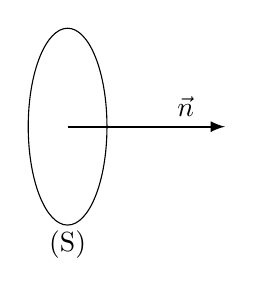
\begin{tikzpicture}[scale=1]  
                    % \helpgrid{3}{3}
                    \draw (0,0) ellipse (0.5 and 1.25);
                    \draw [-latex, thick] (0,0) --++(2,0) node [above, pos=0.75] {$\vec{n}$};
                    \node at (0,-1.5) {(S)};
                \end{tikzpicture}
                \caption{Courant algébrique traversant une surface orientée.}    
                \label{fig:courant_algebrique_traversant_surface_orientee}
            \end{figure}

            Le courant $i(t)$ est alors défini par 
            \begin{equation}
                \boxed{
                    \delta Q=i(t)\rmd t.
                }
            \end{equation}

            Son unité est \si{\ampere}=\si{\coulomb\per\second}. C'est la charge algébrique traversant la surface orientée (S) par unité de temps.

        \subsubsection{Densité de courant}

            \paragraph{Cas à une dimension et un seul type de porteur libre.}

                On considère qu'il y a $n$ porteur libres par metre cube, $q$ est la charge algébrique d'un porteur, $\vec{v}$ est la vitesse d'ensemble, qui est uniforme et perpendiculaire à (S), voir la Figure~\ref{fig:densite_courant_modele_introductif}.

                \begin{figure}
                    \centering
                    \tikzsetnextfilename{densite_courant_modele_introductif}
                    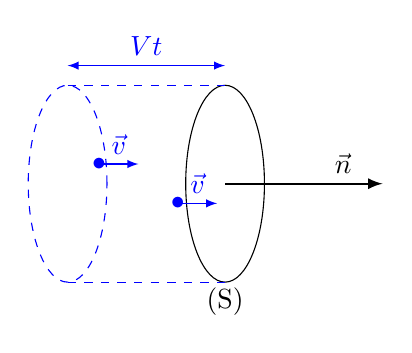
\begin{tikzpicture}[scale=1]  
                        % \helpgrid{3}{3}
                        \draw (0,0) ellipse (0.5 and 1.25);
                        \draw[dashed, blue] (-2,0) ellipse (0.5 and 1.25);
                        \draw[latex-latex,draw=blue,text=blue] (-2,1.5)--(0,1.5) node [above, midway] {$V\rmd t$};
                        \draw[dashed, draw=blue] (-2,1.25)--(0,1.25);
                        \draw[dashed, draw=blue] (-2,-1.25)--(0,-1.25);
                        \draw[-latex,draw=blue,text=blue] (-1.6,0.25)--++(0.5,0) node [above,midway] {$\vec{v}$} node [pos=0] {$\bullet$};
                        \draw[-latex,draw=blue,text=blue] (-0.6,-0.25)--++(0.5,0) node [above,midway] {$\vec{v}$} node [pos=0] {$\bullet$};
                        \draw [-latex, thick] (0,0) --++(2,0) node [above, pos=0.75] {$\vec{n}$};
                        \node at (0,-1.5) {(S)};
                    \end{tikzpicture}
                    \caption{Densité de courant $\vec{j}$ : modèle introductif.}    
                    \label{fig:densite_courant_modele_introductif}
                \end{figure}

                Le nombre $\delta N$ de porteurs traversant (S) pendant $\rmd t$ est 
                \begin{equation}
                    \delta N=n S v\rmd t=n\vec{v}\cdot(S\vec{n})\rmd t,
                \end{equation}
                d'où 
                \begin{equation}
                    \delta Q=\delta N\times q=nq\vec{v}\cdot(S\vec{n})\rmd t
                \end{equation}
                et finalement 
                \begin{equation}
                    \boxed{
                        i=nq\vec{v}\cdot\vec{n}S=\vec{j}\cdot(S\vec{n}),
                    }
                \end{equation}
                où $\vec{j}=nq\vec{v}$ est la \textbf{densité de courant}, d'unité \si{\ampere\per\metre\squared}.

                Dans le cas où la vitesse n'est pas perpendiculaire à (S), le calcul reste le même (en prenant bien en compte le produit scalaire avec la normale extérieure $\vec{n}$).

            \paragraph{Définition de $\vec{j}$.}

                De manière générale, on définit la densité de courant $\vec{j}(\vec{r},t)$ par 
                \begin{equation}
                    \boxed{
                        i_s(t)\coloneqq\iint_{S}\vec{j}(\vec{r},t)\cdot\vec{n}\rmd S.
                    }
                \end{equation}

                $i_s(t)$ est le flux de $\vec{j}$ à travers la surface $S$.

        \subsubsection{Expression de $\vec{j}$ dans différents milieux conducteurs}

            \paragraph{Métal.} 
            
                Les électrons libres génèrent une densité de courant 
                \begin{equation}
                    \vec{j}=-n\rme \langle \vec{v}\rangle.
                \end{equation}

                Dans un fil de cuivre pour 1~\si{\ampere} et une longueur 2~\si{\milli\metre}, on a 
                \begin{equation}
                    n_\rme\sim\frac{1}{(\text{qq}.10^{10})^{3}}\sim 10^{29}~\si{\per\metre\cubed}.
                \end{equation}
                Ainsi, l'ordre de grandeur de la vitesse des électrons dans le métal est 
                \begin{equation}
                    \langle v\rangle \sim \frac{1}{10^{29}\times10^{19}\times 2.10^{-6}}\sim3.10^{-5}~\si{\metre\per\second}.
                \end{equation}

                En considérant les électrons comme des particules classiques indépendantes, on a 
                \begin{equation}
                    \frac{1}{2}m\vec{v}^{2}=\frac{3}{2}k_b T,
                \end{equation}
                avec $k_B=R/\mathcal{N}_A\approx 1.38.10^{-23}~\si{\joule\per\kelvin}$.

                Ainsi,
                \begin{equation}
                    v=\sqrt[]{\frac{3k_B T}{m}}\sim 10^{5}~\si{\metre\per\second},
                \end{equation}
                pour $m=0.9^{-30~\si{\kilo\gram}}$ et $T=300~\si{\kelvin}$.

            \paragraph{Semi-conducteur.} 

                On a 
                \begin{equation}
                    \vec{j}=n_t\rme\langle \vec{v_t}\rangle-n_\rme\rme\langle\vec{v}_\rme\rangle.
                \end{equation}

            \paragraph{Solution de \ce{NaCl}.}

                On a 
                \begin{equation}
                    \vec{j}=n_{\ce{Na+}}\rme\langle\vec{v}_{\ce{Na+}}\rangle-n_{\ce{Cl-}}\rme\langle\vec{v}_{\ce{Cl-}}\rangle.
                \end{equation}

            Finalement, on a 
            \begin{equation}
                \boxed{
                    \vec{j}=\sum_{\substack{\neq\text{ types}\\\text{de particules libres}}}n_k q_k\langle \vec{v}_k\rangle.
                }
            \end{equation}